\section{Experimental Results}
\label{sec:experiment-results}
In this section, we explore a variety of GAD experiments. As anomaly detection is an unsupervised learning problem, model evaluation is highly challenging. {  We employ anomaly injection where known group anomalies are injected into  real-world image datasets. The performances of DGMs are evaluated against state-of-the-art GAD methods using area under precision-recall curve (AUPRC) and area under receiver operating characteristic curve (AUROC) metrics. AUPRC  is  more appropriate  than AUROC for binary classification under class imbalanced datasets such as in GAD applications~\cite{Davis:2006}.
However in the following experiments, a high AUPRC score usually indicates the effectiveness of accurately identifying regular groups while AUROC accounts for the false positive rate of detection methods. %detection of group anomalies
}

\subsection{Synthetic Data: Rotated Gaussians }
Firstly we generate synthetic data where
regular behaviour consists of  bivariate Gaussian samples while anomalous groups have rotated covariance structures. %$\big({X}_{i1}(t),{X}_{i2}(t) \big)_{i=1}^N \sim \mathcal{N}\big ({\boldsymbol \mu(t)},\boldsymbol \Sigma(t) \big)$. In this experiment,
We generate synthetic data with number of groups $M=550$ and $M=5050$. 50 anomalous groups are injected with correlation $\rho =-0.7$ while the rest of the regular group distributions have  correlation $\rho =0.7$.  The mean vectors are randomly sampled from uniform distributions %with $  \mu_1(t), \, \mu_2(t) \sim \mathcal{U}(0,1)$ for $t \in [1,T]$.
 while covariances of group distributions are given by
 \begin{equation}
  \boldsymbol\Sigma_m=\left\{
  \begin{array}{@{}ll@{}}
  \;
\begin{pmatrix}
     0.2 & 0.14 \\
  0.14 & 0.2
  \end{pmatrix}, & m=1,2,\dots,500 \\[5mm]
  \;  \small \begin{pmatrix}
     0.2 & -0.14 \\
  -0.14 & 0.2
  \end{pmatrix}, &m=501,502,\dots,550 \end{array}\right.
    \label{changecovariance}
\end{equation}
with each group having $N_m = 1536$ observations.
{  Since we configured the proposed DGMs with an architecture suitable  for $32\times 32$ pixels for 3 dimensions (red, green, blue), our dataset is constructed such that each group has bivariate observations with a total of $N_m \times 2 = 3072$ values. }

% Equivalently, this GSP over $[1,T/2]$ has a linear correlation between observations of $\rho =0.5$ whereas there is an increase in   correlation  with $\rho =0.95$ for $(T/2,T]$. \\
% detecting tigers within cats


\textbf{Parameter settings}:
GAD methods are applied on the raw data with various parameter settings.
MGM is trained with $T=1$ regular scene types and $L=3$ as the number of Gaussian mixtures. The expected proportion of group anomalies as true proportion in OCSMM and OCSVM is set to  $\nu = 50/M$ where $M= 550$ or $M= 5050$. In addition, OCSVM is applied by treating each group as a single high-dimensional vector.

\textbf{Results}: Table \ref{tbl:syn} illustrates the results of detecting distribution-based group anomalies for different { number of groups}. For smaller {  number of groups} $M= 550$, state-of-the-art GAD methods achieve a higher performance  than DGMs however for a larger training set with $M= 5050$, deep generative models achieve the highest performance. This conveys that DGMs require larger {  number of group} observations in order to train an appropriate model. { AAE and VAE attain similar results for both synthetic datasets.}

\begin{table*}
    \centering
    \scalebox{1}{
    \begin{tabular}{|c|c|c|c|c|c|c|}
        \hline
        \multirow{2}{*}{Methods} &
        \multicolumn{2}{c|}{\bf { M=550}} &
            \multicolumn{2}{c|}{\bf { M=5050}}
        \\
        \cline{2-5}
        &AUPRC & AUROC &AUPRC & AUROC
          \\
        \hline
        AAE &$0.9060$ &$0.5000$ &\cellcolor{gray!25}$1.0000$ &\cellcolor{gray!25}$1.0000$ \\
        VAE &$0.9001$ &$0.5003$ &\cellcolor{gray!25}$1.0000$&\cellcolor{gray!25}$1.0000$ \\
%         CAE &$0.9070$ &$0.5019$ &$0.9989$&$0.9979$\\
        \midrule
        MGM&\cellcolor{gray!25}$0.9781$ &\cellcolor{gray!25}$0.8180$
           &$0.9978$ &$0.8221$\\
        OCSMM&$0.9426$ &$0.6097$%  &$0.0000$
                  &$0.9943$ &$0.6295$
        \\
        OCSVM&$0.9211$ &$0.5008$&$0.9898$ &$0.5310$%  &$0.0000$
        \\
        \hline
\end{tabular}}
       \vspace{2mm}
        \caption{Results for detecting rotated Gaussian distributions in synthetic datasets where % the first two rows contains deep generative models (AAE and VAE) while other techniques are state-of-the-art GAD methods.
        AAE and VAE attain poor detection results for smaller datasets while they achieve highest performances (as highlighted in gray) for a larger number of groups.  }
    \label{tbl:syn}
\end{table*}

\subsection{Detecting tigers within cat images }
\label{sec:tigerDetect}
%In this section we provide empirical results produced by DNN on synthetic and real data. We show that DNN outperforms several sate-of-the-art competitors in the group anomaly detection task.
Firstly we explore the detection of point-based group anomalies (or image anomalies) by injecting 50 anomalous images of tigers among 5000 cat images.
From Figure~\ref{fig:GAD} (a), the visual features of cats are considered as regular behaviour while  characteristics of tigers are anomalous. The goal is to correctly detect images of tigers (point-based group anomalies) in an unsupervised manner.

\textbf{Parameter settings}:
In this experiment, HOG extracts visual features as inputs for GAD methods. MGM is trained with $T=1$ regular cat type and $L=3$ as the number of mixtures. Parameters in OCSMM and OCSVM are set to  $\nu$ = 50/5050 and OCSVM is applied with $k$-means ($k=40$). Following the success of the Batch Normalisation architecture~\cite{ioffe2015batch} and Exponential Linear Units (elu)~\cite{clevert2015fast}, we have found that convolutional+batch-normalisation+elu layers for DGMs provide a better representation of convolutional filters. Hence, in this experiment the autoencoder of both AAE and VAE adopts four layers of (conv-batch-normalisation-elu) in the encoder part and as well as in the decoder portion of the network. AAE network parameters such as (number of filter, filter size, strides) are chosen to be (16,3,1) for first and second layers while (32,3,1) for third and fourth layers of both encoder and decoder layers. The middle hidden layer size is set to be same as rank $K = 64$ and the model is trained using Adam~\cite{kingma2014adam}. The decoding layer uses sigmoid function in order to capture the non-linearity characteristics from  latent representations produced by the hidden layer.  Similar parameter settings are selected for DGMs in subsequent experiments.


{
\textbf{Results}:
From Table  \ref{tablesummary}, AAE attains the highest AUROC value of 0.9906 while OCSMM achieves a AUPRC of 0.9941. MGM, OCSMM, OCSVM are associated with high AUPRC as  regular groups are correctly identified but their low AUROC scores indicate poor detection of group anomalies. Figure  \ref{fig:results-cifar} (a) further investigates the top 10 anomalous images detected by these methods and finds that AAE correctly detects all images of tigers while OCSMM erroneously captures regular cat images.
}


% detecting cats with dogs
\subsection{Detecting cats and dogs }
We further investigate GAD  %of distribution-based group anomalies
where images of a single cat and dog are considered as regular groups while  images with both cats and dogs are distribution-based group anomalies.   The constructed dataset consists of 5050 images; 2500 single cats, 2500 single dogs and 50 images of  cats and dogs together. % Examples of anomalous images containing  cats and dogs together are previously illustrated in Figure~\ref{fig:GAD}(B).
As previously illustrated in Figure~\ref{fig:GAD} (b), our goal is to detect all images with irregular mixtures of cats and dogs in an unsupervised manner.

% Results for Detecting Cats and Rotated Cats along with detecting Cats together with Dogs.
\textbf{Parameter settings}:
In this experiment, HOG extracts visual features as inputs for GAD methods.
MGM is trained with $T=2$ regular cat type and $L=3$ as the number of mixtures while  OCSVM is applied with $k$-means ($k=30$).

{
\textbf{Results}:
Table  \ref{tablesummary} highlights (in gray) that AEE achieves the highest  AUPRC and AUROC values. %AAE and VAE achieve similar detection performances with AUROC of 1 and 0.9999 respectively. %%%  Why are they similar? Can we know?
Other state-of-the-art GAD methods attain high AUPRC however AUROC values are relatively low. From Figure  \ref{fig:results-cifar} (a), the top 10 anomalous images with both cats and dogs are correctly detected by AAE while OCSMM erroneously captures regular cat images. In fact, OCSMM incorrectly but consistently detects regular cats with similar results to subsection~\ref{sec:tigerDetect}.

}







\subsection{Discovering rotated entities }
We now explore the detection of distribution-based group anomalies with  5000  regular cat images and 50 images of rotated cats. As illustrated in Figure~\ref{fig:GAD} (a), images of rotated cats are anomalous  compared to regular images of cats. Our goal is to detect all rotated cats in an unsupervised manner.

\textbf{Parameter settings}:
In this experiment involving rotated entities, HOG extracts visual features  because SIFT is rotation invariant. MGM is trained with $T=1$ regular cat type and $L=3$ mixtures  while OCSVM is applied with $k$-means ($k=40$).  %For the DGMs, the network parameters follows similar settings to subsection \ref{sec:tigerDetect}. % previous experiment of detecting tigers within cats images.

{
\textbf{Results}:
 In  Table  \ref{tablesummary}, AAE and VAE achieve the highest AUROC with AAE having slightly better detection results. MGM, OCSMM and OCSVM achieve a high AUPRC but low AUROC. Figure \ref{fig:results-rotatedcatsandscene} (a) illustrates the  top 10 most anomalous groups where AAE correctly detects images containing rotated cats while MGM incorrectly identifies regular cats as anomalous. }


\begin{figure}[!t]
     \begin{subfigure}[b]{1\textwidth}
   \centering
   {\includegraphics[scale=0.50]%{catswithrotatedcats}}
{Tigers}}
\caption{Tigers within cat images from {\tt cifar-10} dataset.}
        \end{subfigure}%
        \hfill
        \vspace{2mm}
     \begin{subfigure}[b]{1\textwidth}
\centering
   {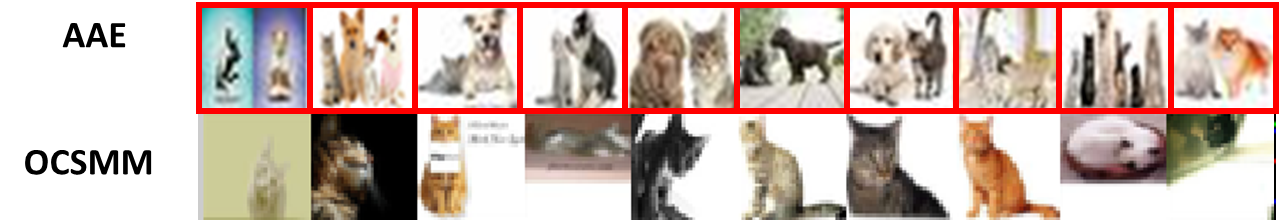
\includegraphics[scale=0.50]{CatsAndDogs}}
\caption{Images of cats and  dogs within single cat and dog images using {\tt cifar-10} dataset.}
        \end{subfigure}%
    \caption{
    Top 10 anomalous groups are presented for AAE and the best GAD method respectively where red boxes outlining images represent true group anomalies.
    %Red boxes around images  represent correctly detected group anomalies as shown in (a) and (b).
    AAE  has an accurate detection of anomalous tigers injected into the {\tt cifar-10} dataset as well as for anomalous images of both cats and dogs. On the other hand, OCSMM consistently but erroneously identifies similar cat images as the most anomalous groups.
    }
    \label{fig:results-cifar}
\end{figure}




% Detecting Stitched scene images.
\subsection{Detecting stitched scene images}
A scene image dataset is also explored where %the two datasets described in Section \ref{sec:experiment-setup}.
 100 images from each category ``inside city”, ``mountain" and ``coast”. 66 group anomalies are added where images are stitched from  two scene categories. % These 300 images are randomly divided: 80\% are used for training and the rest for testing.
% We created anomalies by stitching random regular images from two  categories.
Illustrations are provided in Figure~\ref{fig:GAD} (c) where a stitched image may contain half coast and half city street view. These anomalies are challenging to detect since they have the same local features as regular images however as a collection, they are anomalous.  Our objective is detect stitched scene images in an unsupervised manner.

\textbf{Parameter settings}:
State-of-the-art GAD methods utilise SIFT feature extraction in this experiment. MGM is trained with $T=3$ regular scene types and $L=4$ Gaussian mixtures while %. The expected proportion of group anomalies as true proportion in OCSMM and OCSVMM is set to  $\nu$ = 66/366 where
OCSVM is applied with $k$-means ($k=10$). The scene image dimensions are rescaled
to enable the application of an identical architecture for DGMs as implemented in previous experiments. %
The parameter settings for both AAE and VAE  follows setup as described in Section~\ref{sec:tigerDetect}.

{
\textbf{Results}:
In Table  \ref{tablesummary}, OCSMM achieves the highest AUROC score  %attains the highest performance with AUROC of 0.7162  while AAE has a AUPRC of 0.9449.
%Many GAD methods outperform DGMs in this experiment as
while DGMs are less effective in detecting distribution-based group anomalies in this experiment. We suppose that this is because  only $M=366$ groups are available for training in the  {\tt scene} dataset as  compared to $M=5050$ groups in previous experiments.  Figure  \ref{fig:results-rotatedcatsandscene}   (b) displays the top 10 most anomalous images where OCSMM achieves a better detection results % of distribution-based group anomalies
than AAE.
}

\begin{figure}[!t]
    \centering
 \begin{subfigure}[b]{1\textwidth}
\centering
   {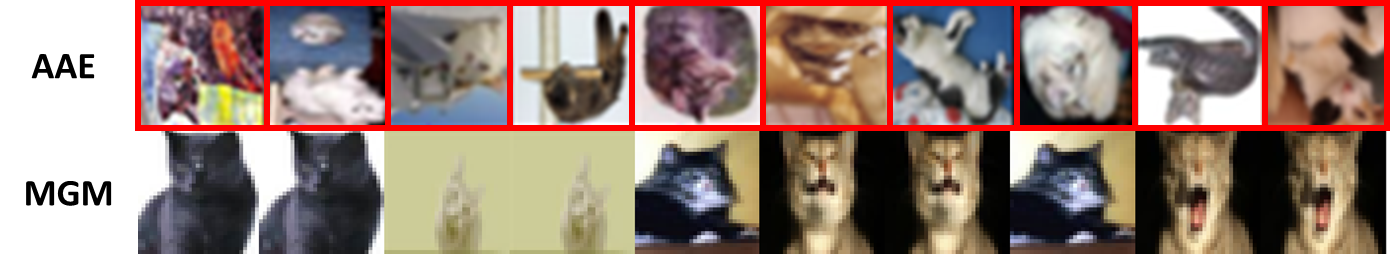
\includegraphics[scale=0.47]{RotatedCats}}
\caption{Rotated cats  amongst regular cats in the {\tt cifar-10} dataset. }
 \end{subfigure}%
 \hfill \vspace{2mm}
 \begin{subfigure}[b]{1\textwidth}
\centering
 {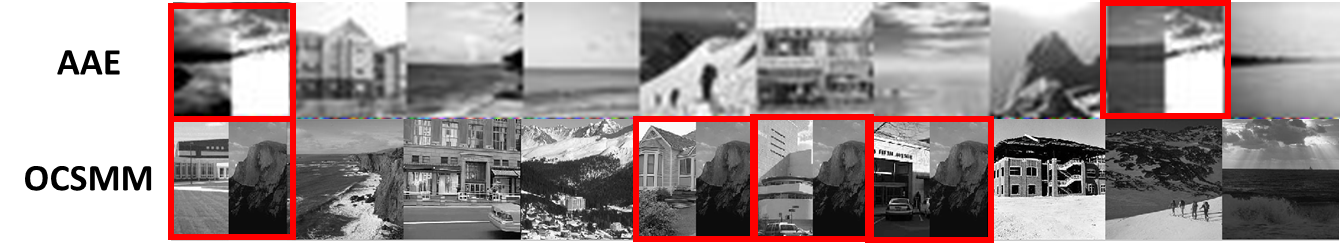
\includegraphics[scale=0.5]{Scene}}
\caption{Stitched Images amongst the {\tt scene} dataset.}
        \end{subfigure}%
   \caption{Top 10 anomalous groups are presented where red boxes outlining images  represent true group anomalies in the given datasets. AAE performs well in (a) with number of groups $M=5050$ however does not effectively detect group anomalies in (b) where number of groups is $M=366$.  MGM is unable to correctly detect any rotated cats while OSCMM is able to group anomalies in the {\tt scene} dataset.
   }
    \label{fig:results-rotatedcatsandscene}
\end{figure}



\subsection{ Results Summary and Discussion}

Table  ~\ref{tablesummary} summarises the performance of detection methods in
%DGMs and state-of-the-art GAD methods for
 our experiments.
AAE usually achieves better results than VAE as AAE has the  advantage of the embedding coverage in the latent space~\cite{makhzani2015adversarial}.  AAE enforces a better mapping of input variables to embedding space and hence captures more robust input features.
DGMs have a significantly worse performance on  {\tt synthetic} and {\tt scene} datasets due to the small number of groups. A high detection performance is achieved for larger number of groups with {\tt cifar-10} and {\tt Pixabay} data experiments.
 Overall, given a sufficient number of group observations for training, DGMs are effective in detecting group anomalies however poor detection occurs for datasets with a small number of groups.







\begin{table*}
   % \centering
        \setlength{\tabcolsep}{1.2mm}
    \scalebox{1}{
    \begin{tabular}{|c|c|c|c|c|c|c|c|c|c|c|}

        \hline
        \multirow{2}{*}{Methods} &
        \multicolumn{2}{c|}{\bf {\small    Tigers }}  &
                \multicolumn{2}{c|}{\bf {\small Cats and Dogs }} &
                \multicolumn{2}{c|}{\bf {\small Rotated Cats}} &
                                  \multicolumn{2}{c|}{\bf {\small Scene }} \\[1mm]
        \cline{2-9}
     &AUPRC & AUROC        & AUPRC & AUROC      &AUPRC & AUROC        & AUPRC & AUROC
        \\
        \hline
        \multirow{4}{*}{}
        AAE& $0.9449$ &\cellcolor{gray!25} $0.9906$
         &\cellcolor{gray!25}$1.0000$ &\cellcolor{gray!25}$1.0000$
            &\cellcolor{gray!25}$1.0000$ &\cellcolor{gray!25}$1.0000$
        & \cellcolor{gray!25} 0.9449 & 0.5906
        \\
          %      AAE\cite{chalapathy2017robust}&\cellcolor{gray!25}$1.0000$ &\cellcolor{gray!25}$1.0000$
                %&\cellcolor{gray!25}$1.0000$                   &\cellcolor{gray!25}$1.0000$ &\cellcolor{gray!25}$1.0000$%&\cellcolor{gray!25}$1.0000$           \\
%         CAE & &
%         &$0.9998$ &$0.9999$
%          &$0.9999$ &$0.9999$
%         & &
%         \\
        VAE&$0.9786$ &$0.9092$ % &$0.9997$
               &$0.9998$ &$0.9999$
        &$0.9999$ &$0.9999$%&$0.9999$
                  &$0.8786$ &$0.3092$
        \\
        \midrule
        MGM & $0.9881$ & $0.5740$
        &0.9906 & 0.5377
        &$0.9919$ &$0.6240$ % &$0.0000$
               &0.8835 & 0.6639
        \\
        OCSMM
             &\cellcolor{gray!25} $0.9941$ &$0.6461$%  &$0.0000$
        & 0.9930 & 0.5876
        &$0.9917$ &$0.6128$%  &$0.0000$
             &$0.9140$ &\cellcolor{gray!25} $0.7162$%  &$0.0000$
        \\
        OCSVM
        & 0.9909 & 0.5474
        & 0.9916 & 0.5549
        &$0.9894$ &$0.5568$%  &$0.0000$
        & 0.8650 & 0.5733
        \\
        \hline
\end{tabular}}
       \vspace{2mm}
        \caption{Summary of results for various data experiments where first two rows contains deep generative models and other techniques are state-of-the-art GAD methods. The highest values of performance metrics are shaded in gray.}
    \label{tablesummary}
\end{table*}


{\bf Comparison of training times:}
\label{sec:runtime}
We add a final remark about applying the proposed DGMs on  GAD problems in terms of computational time and training efficiency.
For example, including the time taken to calculate SIFT features on the small-scale {\tt scene} dataset, MGM takes 42.8 seconds for training, 3.74 minutes to train OCSMM and 27.9 seconds for OCSVM. In comparison, the computational times for our AAE and VAE are  6.5 minutes and 8.5 minutes respectively. %All the experiments involving DGMs were conducted on a MacBook Pro equipped with an Intel Core i7 at 2.2 GHz, 16 GB of RAM (DDR3 1600 MHz).
 The ability to leverage recent advances in deep learning as part of our optimisation (e.g. training models on a GPU) is  a salient feature of our approach. We also note that MGM and OCSMM are faster to train on small-scale datasets however they suffer from at least $O(N^2)$ complexity for total number of observations $N$. %; for example, it takes over an hour to train on the {\tt cifar-10} dataset.
It is plausible that one could leverage recent advances in fast approximations of kernel methods~\cite{Lopez-Paz:2014} for OCSMM and studying these would be of interest in future work.









